\documentclass{article}
\usepackage[utf8]{inputenc}
\usepackage[backend=biber,style=ieee]{biblatex}  
\usepackage{float}

% needed for specifying column with and centering at the same time
\usepackage{array}
\newcolumntype{C}[1]{>{\centering\arraybackslash}p{#1}}

% needed for inserting images
\usepackage{graphicx}
\graphicspath{ {./images/} }

\addbibresource{literatur.bib}

\title{Feature Extraction Report}
\author{Philipp Steinwender $^{1}$ \\
    \small $^{1}$Student at Graz University of Technology
}
\date{January 2023}

\begin{document}

\maketitle

\begin{abstract}
Classification of EEG data is a very hard task and involves often good data-preprocessing, feature-extraction and a correctly selected and trained model. This report focuses on the Feature-Engineering aspect and compares different feature extraction methods. The resulting performance is documented and discussed shortly. It should provide an basic overview about possible extraction methods and how they perform on EEG data during motor imagery.
\end{abstract} \hspace{10pt}
\newpage
\tableofcontents
\newpage

\section{Introduction}
This report describes different methods to extract features of EEG data and furthermore train a model. Performance results of different extracted features are shown, described and compared.
\section{Materials}
In order to train and compare results, the BCI competition IV 2a dataset was used. This dataset contains motor imagery data which was recorded by 22 EEG channels. It is a 4-Class motor imagery classification problem \parencite{10.3389/fnins.2012.00055, brunner2008bci}.
The complete report is created based on results generated by a model written in matlab \parencite{Steinwender_Research_Software_2022}.

\section{Methods}
Improving classification accuracies by using a extraction method is desirable. In this section different extraction methods of signals are proposed. This extraction techniques will be applied to EEG data. All these different techniques will either operate in time- or frequency-domain.

\subsection{Autoregressive methods}
Autoregressive models (Ar-Models) try to predict the future based on previous data-points. The influence of the past can be changed based on the order of the Ar-Model. Higher orders result in a larger impact of the past into the future prediction. Therefore selecting the correct order is key for a good performing Ar-Model. The following Ar-Models are used by the Ar-Extractor:
\begin{itemize}
    \item Autoregressive all-pole model parameters — covariance method (arcov) \parencite{arcov}
    \item Autoregressive all-pole model parameters — Yule-Walker method (aryule) \parencite{aryule}
    \item Autoregressive all-pole model parameters — Burg’s method (arburg) \parencite{arburg}
    \item Autoregressive all-pole model parameters — modified covariance method (armcov) \parencite{armcov}
\end{itemize}
\subsection{Power spectral density (psd)} \label{power-spectral-density}
The psd describes the power distribution of the signal over the frequencies. First of all the psd gets calculated based on the recorded raw EEG data. In order to calculate the psd different psd methods (section \ref{psd-methods}) will be used and compared in this report. After calculating the psd the frequency bands get extracted. An overview about the extracted frequency bands can be found at table \ref{tbl:frequency-bands}.
\begin{table}[H]
 \centering
 \begin{tabular}{|c|c|}
 \hline
   \textbf{Frequency-Band-Name}  & \textbf{Frequency-Band-Interval [Hz]} \\\hline
   delta            & 0.1 - 3.5             \\
   theta            & 4 - 7.5             \\
   alpha            & 8 - 12.5             \\
   beta             & 13 - 29.5 \\
   gamma            & 30 - 60 \\
   high-gamma       & 60.5 - 100 \\
   broad            & 0.1 - 100\\\hline
 \end{tabular}

 \caption{frequency bands}
 \label{tbl:frequency-bands}
 % Verweis im Text mittels \ref{tbl:frequency-bands}
\end{table}

After that statistic features (section \ref{statistic-features}) are extracted of each band. This features are then supplied to the classifier.

\subsubsection{Psd-Methods} \label{psd-methods}
For calculating the psd, multiple methods are possible. In this section, a small overview about the used methods is provided.
\begin{itemize}
    \item Welch’s power spectral density estimate (pwelch) \parencite{pwelch}
    \item Autoregressive power spectral density estimate — covariance method (pcov) \parencite{pcov}
    \item Autoregressive power spectral density estimate — modified covariance method (pmcov) \parencite{pmcov}
    \item Autoregressive power spectral density estimate — Burg’s method (pburg) \parencite{pburg}
    \item Autoregressive power spectral density estimate — Yule-Walker method (pyulear) \parencite{pyulear}
\end{itemize}

\subsection{Statistic features} \label{statistic-features}
Extracting statistical features helps to understand and describe data. The following statistical features are calculated and applied to EEG-data.  
\begin{itemize}
    \item \textbf{min:} Minimum of the data-vector
    \item \textbf{max:} Maximum of the data-vector
    \item \textbf{mean:} Mean of the data-vector
    \item \textbf{median:} Median of the data-vector
    \item \textbf{standard deviation:} Standard deviation of the data-vector
    \item \textbf{var:} Variance of the data-vector
    \item \textbf{kurtosis:} Kurtosis of the data-vector
    \item \textbf{skewness:} Skewness of the data-vector
    \item \textbf{prctile:} 50\% percentile of the data-vector
    \item \textbf{entropy:} Entropy of the data-vector
    \item \textbf{spectral entropy:} Spectral entropy of the data-vector
    \item \textbf{slope:} Calculates the slope between the first and the last data-point of the window-size vector.
\end{itemize}

\subsection{Lyapunov Exponentes}
Lyapunov exponents provide insights into the behavior of a dynamical system. For feature comparison lyapunov exponents are calculated for time- and frequency-domain data.

\subsection{Wavelet transformation}
The wavelet transformation is a mathematical tool to analyse signals. It performs very good for nonstationary signals (signals that vary over time) compared to other transformation methods. 
\begin{itemize}
    \item Wavelet Entropy \parencite{wentropy}
    \item Multiscale variance of maximal overlap discrete wavelet transform \parencite{wvariance}
    \item Multiscale correlation using the maximal overlap discrete wavelet transform \parencite{wcorrelation}
\end{itemize}

\subsection{Window size}
Each extractor operates with a given window size. The window size represents a number of signal samples. Small window sizes reduce the impact of past signal information. Whereas larger window sizes involves more signal information from a previous time point. Choosing an appropriate window size is necessary to achieve a high classification accuracy.

\subsection{Data preprocessing}
Preprocessing the data by subsampling the raw EEG-signal changes performance of the classifier. It reduces the bandwith of the signal and therefore classification speed is increased due to reduced number of data-points. Additionally, artifact trials are removed before classification. The artifact-trials are already predetermined by the dataset.

\subsection{Classifier}
The current used classifier is the linear discriminant analysis classifier (LDA). LDA looks for a linear explanation that fits the data best. LDA classifier is trained and compared with different input features.

\section{Results}
In the following sections, results of testing the implemented extractors based on different parameters are shown. All different used parameters are described in the corresponding sections. Only the best configurations of each extractor are listed. For all other tested parameters checkout the saved figures or run the code manually \parencite{Steinwender_Research_Figures_2022}.

\subsection{Statistic-Extractor}
Statistic measures are applied to raw EEG data (in time-domain) for each window size. Currently only one statistic feature is extracted for easier comparison. Several statistical measures where tested and compared. All allowed statistical features can be found in section \ref{statistic-features}.

\begin{table}[H]
 \centering
 \begin{tabular}{|C{0.15\linewidth}|C{0.05\linewidth}|C{0.12\linewidth}|C{0.08\linewidth}|C{0.14\linewidth}|c|}
 \hline
   \textbf{statistic measure}  & \textbf{fs [Hz]} & \centering\textbf{Window Size} & \textbf{Time [s]} & \textbf{Accuracy [\%]} & \textbf{Kappa} \\\hline
   mean    & 50  & 20  & 1.2 & 49.88 & 0.332 \\
   mean    & 250 & 100 & 1.2 & 49.13 & 0.322 \\
   mean    & 25  & 10  & 1.2 & 48.77 & 0.317 \\
   min     & 50  & 20  & 1.2 & 44.65 & 0.263 \\
   min     & 250 & 100 & 1.2 & 43.62 & 0.249 \\
   slope   & 250 & 100 & 0.8 & 41.38 & 0.217 \\
   std     & 250 & 100 & 1.2 & 41.35 & 0.217 \\
   std     & 50  & 20  & 1.2 & 41.03 & 0.214 \\
   prctile & 250 & 100 & 0.8 & 40.97 & 0.212 \\
   median  & 250 & 100 & 0.8 & 40.97 & 0.212 \\
   slope   & 25  & 10  & 0.8 & 40.67 & 0.208 \\
   min     & 25  & 10  & 1.2 & 40.60 & 0.209 \\
   prctile & 25  & 10  & 0.8 & 40.59 & 0.207 \\
   median  & 25  & 10  & 0.8 & 40.59 & 0.207 \\\hline
 \end{tabular}
 \caption{Statistic-Extractor performance comparison of different parameters}
 \label{tbl:statistic-feature-comparison-table}
 % Verweis im Text mittels \ref{tbl:statistic-feature-comparison-table}
\end{table}

\begin{figure}[H]
    \centering
    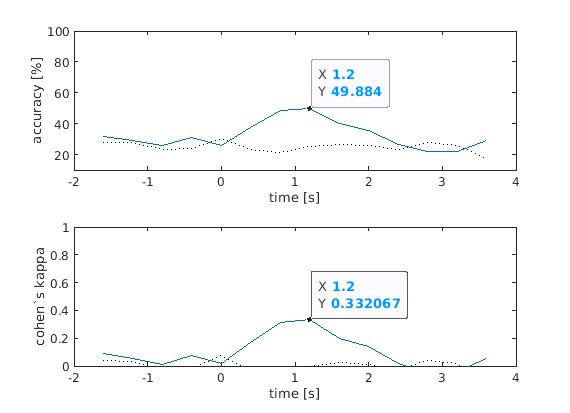
\includegraphics[width=\textwidth]{images/49.88-50hz-20-statistic-mean.jpg}
    \caption{This chart contains the performance measures of the Statistic-Feature extraction. It uses the mean of the data-points window. This extraction method was tested with fs = 50Hz and a window size of 20 data-points.}
    %\label{fig:my_label}
\end{figure}

Statistic features like min, mean, median, std, prctile and slope perform well. Non promising features are skewness, kurtosis, entropy, spectral-entropy, variance and max.

\subsection{Ar-Extractor}
The Ar-Model was trained with the raw EEG data (in time-domain) and the ar-coefficients of the trained model where used as features. Each model was tested with the following parameters:
\begin{itemize}
    \item \textbf{Method:} The Ar-Model method (arcov, aryule, arburg or armcov)
    \item \textbf{Order:} The Ar-Model order (3, 4, 5, 6)
    \item \textbf{White-Noise:} White noise input variance (true, false)
    \item \textbf{fs:} Different sampling rates are used on the base EEG data. (250Hz, 50Hz, 25Hz)
    \item \textbf{Window Size:} Window sizes are adapted accordingly to the changed sampling rates (100, 20, 10)
\end{itemize}

\begin{table}[H]
 \centering
 \begin{tabular}{|c|C{0.08\linewidth}|C{0.08\linewidth}|C{0.05\linewidth}|C{0.12\linewidth}|C{0.08\linewidth}|C{0.14\linewidth}|c|}
 \hline
   \textbf{Method} & \textbf{Order} & \centering\textbf{White Noise}  & \textbf{fs [Hz]} & \centering\textbf{Window Size} & \textbf{Time [s]} & \textbf{Accuracy [\%]} & \textbf{Kappa} \\\hline
   arcov  & 4 & false & 250 & 100 & 1.2 & 46.87 & 0.291 \\
   arcov  & 3 & true  & 250 & 100 & 1.2 & 46.87 & 0.291 \\
   armcov & 4 & false & 250 & 100 & 1.2 & 46.54 & 0.287 \\
   armcov & 3 & true  & 250 & 100 & 1.2 & 46.54 & 0.287 \\
   arburg & 4 & false & 250 & 100 & 1.2 & 45.39 & 0.271 \\
   arburg & 3 & true  & 250 & 100 & 1.2 & 45.39 & 0.271 \\
   arcov  & 3 & false & 50  & 20  & 1.2 & 44.94 & 0.265 \\
   aryule & 4 & false & 250 & 100 & 1.2 & 43.61 & 0.248 \\
   aryule & 3 & true  & 250 & 100 & 1.2 & 43.61 & 0.248 \\
   aryule & 6 & true  & 250 & 100 & 1.2 & 43.54 & 0.246 \\\hline
 \end{tabular}
 \caption{Ar-Extractor performance comparison of different parameters}
 \label{tbl:ar-feature-comparison-table}
 % Verweis im Text mittels \ref{tbl:ar-feature-comparison-table}
\end{table} 

\begin{figure}[H]
    \centering
    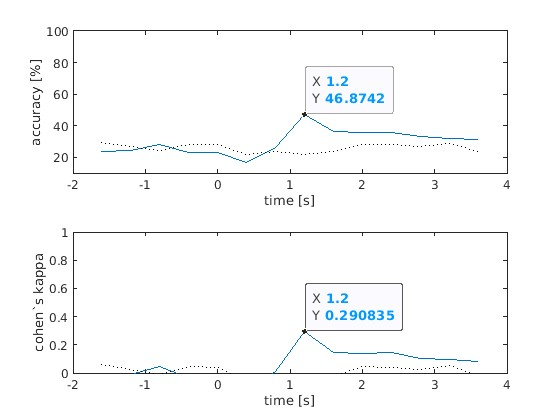
\includegraphics[width=\textwidth]{46.87-250hz-100-ar-arcov-4-false.jpg}
    \caption{This chart contains the performance measures of the Ar-Feature extraction. This model uses the arcov method with an order of 4 and without-white noise. This extraction method was tested with fs = 250Hz and a window size of 100 data-points.}
    %\label{fig:my_label}
\end{figure}

Taking a look at worse parameters shows that higher order ar-extraction performs worse. Subsampling the data influences the classification accuracies and decreases them.

\subsection{Psd-Extractor}

This Extractor uses the welch's power spectrum density estimate and converts the time-domain data-points into the frequency-domain. After that the frequency-domain data is split up into different frequency bands. For each frequency band the statistic extractor extracts one feature. The following parameters are permuted for determining the best configuration:
\begin{itemize}
    \item \textbf{Statistic:} Contains the statistic feature that should be extracted for each frequency band.
    \item \textbf{fs:} Different sampling rates are used on the base EEG data. (250Hz, 50Hz, 25Hz)
    \item \textbf{Window Size:} Window sizes are adapted accordingly to the changed sampling rates (100, 20, 10)
\end{itemize}

\begin{table}[H]
 \centering
 \begin{tabular}{|c|C{0.05\linewidth}|C{0.12\linewidth}|C{0.08\linewidth}|C{0.14\linewidth}|c|}
 \hline
   \textbf{Statistic} & \textbf{fs [Hz]} & \centering\textbf{Window Size} & \textbf{Time [s]} & \textbf{Accuracy [\%]} & \textbf{Kappa} \\\hline
   std      & 250 & 100 & 1.2 & 48.36 & 0.309 \\
   prctile  & 25  & 10  & 1.2 & 47.80 & 0.303 \\
   median   & 25  & 10  & 1.2 & 47.80 & 0.303 \\
   mean     & 25  & 10  & 1.2 & 47.42 & 0.298 \\
   max      & 25  & 10  & 1.2 & 46.68 & 0.288 \\
   min      & 25  & 10  & 1.2 & 46.24 & 0.282 \\
   mean     & 250 & 100 & 1.2 & 45.22 & 0.268 \\
   prctile  & 250 & 100 & 1.2 & 44.60 & 0.260 \\
   median   & 250 & 100 & 1.2 & 44.60 & 0.260 \\
   max      & 250 & 100 & 1.2 & 43.90 & 0.250 \\
   slope    & 250 & 100 & 1.2 & 43.15 & 0.240 \\
   min      & 50  & 20  & 1.2 & 42.29 & 0.230 \\
   min      & 250 & 100 & 1.2 & 42.07 & 0.226 \\
   max      & 50  & 20  & 1.2 & 41.92 & 0.225 \\
   mean     & 50  & 20  & 1.2 & 41.20 & 0.215 \\
   prctile  & 50  & 20  & 1.2 & 40.81 & 0.210 \\
   median   & 50  & 20  & 1.2 & 40.81 & 0.210 \\\hline
 \end{tabular}
 \caption{Psd-Extractor performance comparison of different parameters}
 \label{tbl:psd-feature-comparison-table}
 % Verweis im Text mittels \ref{tbl:psd-feature-comparison-table}
\end{table} 

\begin{figure}[H]
    \centering
    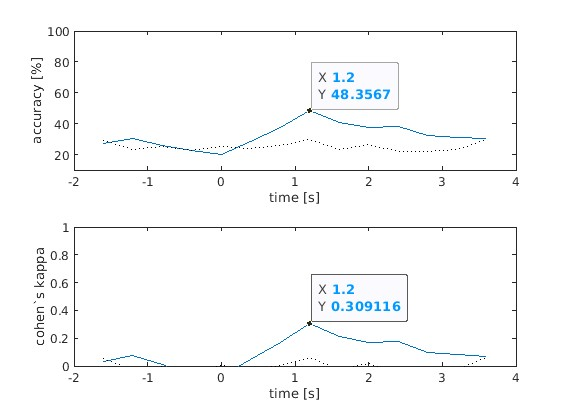
\includegraphics[width=\textwidth]{images/48.36-250hz-100-psd-statistic-std.jpg}
    \caption{This chart contains the performance measures of the Psd-Feature extraction. The std statistic feature is used on top of each frequency band. This extraction method was tested with fs = 250Hz and a window size of 100 data-points.}
    %\label{fig:my_label}
\end{figure}

Min, max, mean, median, std, prctile and slope perform very well. They show high statistical significance. On the other hand, kurtosis, skewness, var, entropy and spectral entropy do not show high or in some cases any significance. Subsampling the data shows in some cases large improvements of performance. Tuning this parameter is very important.

\subsection{Ar-Psd-Extractor}
An Ar-Model estimates the Psd based on the following possible parameterizations:
\begin{itemize}
    \item \textbf{Ar Method:} Contains the Ar-Method for extracting the Psd (pcov, pmcov, pburg, pyulear)
    \item \textbf{Order:} The Ar-Model order (3, 4, 5, 6)
    \item \textbf{Statistic:} Contains the statistic feature that should be extracted for each frequency band.
    \item \textbf{fs:} Different sampling rates are used on the base EEG data. (250Hz, 50Hz, 25Hz)
    \item \textbf{Window Size:} Window sizes are adapted accordingly to the changed sampling rates (100, 20, 10)
\end{itemize}

\begin{table}[H]
 \centering
 \begin{tabular}{|C{0.12\linewidth}|c|c|C{0.05\linewidth}|C{0.12\linewidth}|C{0.08\linewidth}|C{0.14\linewidth}|c|}
 \hline
   \textbf{Ar Method} & \textbf{Order} & \textbf{Statistic} & \textbf{fs [Hz]} & \centering\textbf{Window Size} & \textbf{Time [s]} & \textbf{Accuracy [\%]} & \textbf{Kappa} \\\hline
   pyulear & 6 & min     & 250 & 100 & 1.2 & 53.93 & 0.386 \\
   pmcov   & 6 & max     & 250 & 100 & 1.2 & 52.23 & 0.362 \\
   pburg   & 6 & max     & 250 & 100 & 1.2 & 52.21 & 0.362 \\
   pyulear & 6 & slope   & 250 & 100 & 1.2 & 52.01 & 0.360 \\
   pburg   & 3 & mean    & 50  & 20  & 1.2 & 51.82 & 0.357 \\
   pyulear & 6 & mean    & 250 & 100 & 1.2 & 51.61 & 0.355 \\
   pyulear & 6 & max     & 250 & 100 & 1.2 & 51.56 & 0.354 \\
   pyulear & 5 & prctile & 250 & 100 & 1.2 & 50.84 & 0.344 \\
   pyulear & 5 & median  & 250 & 100 & 1.2 & 50.84 & 0.344 \\
   pmcov   & 5 & mean    & 50  & 20  & 1.2 & 50.70 & 0.342 \\
   pmcov   & 6 & slope   & 250 & 100 & 1.2 & 50.15 & 0.335 \\
   pburg   & 6 & mean    & 250 & 100 & 1.2 & 50.03 & 0.333 \\
   pburg   & 6 & slope   & 250 & 100 & 1.2 & 49.30 & 0.330 \\
   pmcov   & 6 & mean    & 250 & 100 & 1.2 & 49.68 & 0.329 \\
   pyulear & 3 & mean    & 50  & 20  & 1.2 & 49.40 & 0.325 \\
   pmcov   & 6 & std     & 250 & 100 & 1.2 & 49.37 & 0.324 \\\hline
 \end{tabular}
 \caption{Ar-Psd-Extractor performance comparison of different parameters}
 \label{tbl:ar-psd-feature-comparison-table}
 % Verweis im Text mittels \ref{tbl:ar-psd-feature-comparison-table}
\end{table}

\begin{figure}[H]
    \centering
    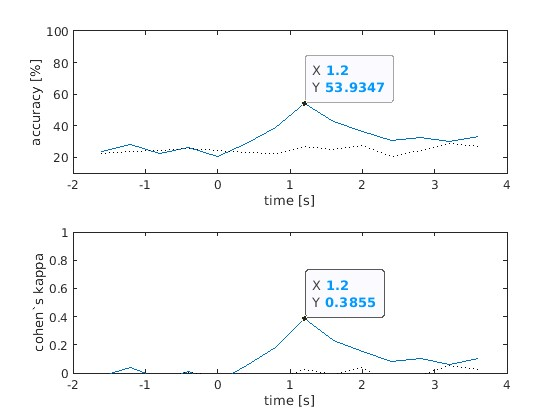
\includegraphics[width=\textwidth]{images/53.93-250hz-100-arPsd-pyulear-6-statistic-min.jpg}
    \caption{This chart contains the performance measures of the Ar-Psd-Feature extraction. It uses the pyulear method of order 6. The min statistic measure gets extracted of the resulting power spectrum bands. This extraction method was tested with fs = 250Hz and a window size of 100 data-points.}
    %\label{fig:my_label}
\end{figure}

Ar-Psd feature extraction shows high statistical significance. High performance statistic parameters were min, max, mean, median, std, prctile and slope. Skewness, kurtosis and var show only low significance. Entropy shows no significance. The overall performance can be increased with the ar-method and the correct order. Every ar-method performed very good if the order is selected correctly. A small trend of the order occurs, it seems that higher order ar-models perform better (on average).

\subsection{Lyapunov-Extractor}
This extractor performs lyapunov-feature-extraction on the time-domain data-points of the given window-size. The following parameters are permuted for determining the best configuration:
\begin{itemize}
    \item \textbf{fs:} Different sampling rates are used on the base eeg data. (250Hz, 50Hz, 25Hz)
    \item \textbf{Window Size:} Window sizes are adapted accordingly to the changed sampling rates (100, 20, 10)
\end{itemize}

\begin{table}[H]
 \centering
 \begin{tabular}{|C{0.05\linewidth}|C{0.12\linewidth}|C{0.08\linewidth}|C{0.14\linewidth}|c|}
 \hline
   \textbf{fs [Hz]} & \centering\textbf{Window Size} & \textbf{Time [s]} & \textbf{Accuracy [\%]} & \textbf{Kappa} \\\hline
   250 & 100 & 2.0 & 33.29 & 0.111 \\
   25  & 10  & 1.6 & 26.80 & 0.024 \\
   50  & 20  & 1.6 & $<$25.0 & - \\\hline
 \end{tabular}
 \caption{Lyapunov-Extractor performance comparison of different parameters}
 \label{tbl:lyapunov-feature-comparison-table}
 % Verweis im Text mittels \ref{tbl:lyapunov-feature-comparison-table}
\end{table} 

\begin{figure}[H]
    \centering
    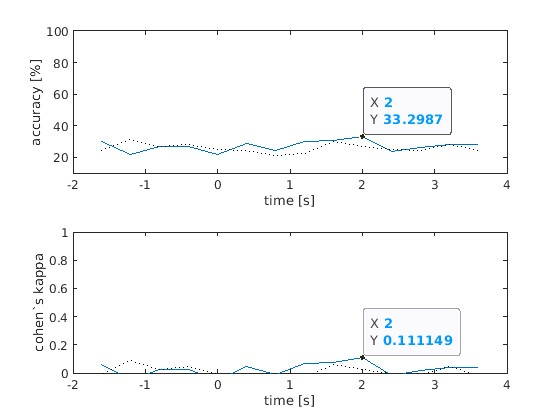
\includegraphics[width=\textwidth]{images/33.30-250hz-100-lyapunov.jpg}
    \caption{This chart contains the performance measures of the Lyapunov-Feature extraction. This extraction method was tested with fs = 250Hz and a window size of 100 data-points.}
    %\label{fig:my_label}
\end{figure}

This feature extraction method does not perform very well. No statistical significance around the time interval 1 - 2 seconds. If the data gets sub-sampled this extraction method performs even worse. Do not use this feature to describe eeg data.

\subsection{Wavelet-Correlation-Extractor}
The wavelet-correlation extraction method calculates the wavelet-correlation of each data-point vector of length=window-size and each different channel. The following parameters are permuted for determining the best configuration: 
\begin{itemize}
    \item \textbf{fs:} Different sampling rates are used on the base eeg data. (250Hz, 50Hz, 25Hz)
    \item \textbf{Window Size:} Window sizes are adapted accordingly to the changed sampling rates (100, 20, 10)
\end{itemize}

\begin{table}[H]
 \centering
 \begin{tabular}{|C{0.05\linewidth}|C{0.12\linewidth}|C{0.08\linewidth}|C{0.14\linewidth}|c|}
 \hline
   \textbf{fs [Hz]} & \centering\textbf{Window Size} & \textbf{Time [s]} & \textbf{Accuracy [\%]} & \textbf{Kappa} \\\hline
   50  & 20  & 1.2 & 50.01 & 0.332 \\
   250 & 100 & 1.2 & 45.73 & 0.276 \\
   25  & 10  & 1.2 & 32.16 & 0.096 \\\hline
 \end{tabular}
 \caption{Wavelet-Correlation-Extractor performance comparison of different parameters}
 \label{tbl:wavelet-correlation-feature-comparison-table}
 % Verweis im Text mittels \ref{tbl:wavelet-correlation-feature-comparison-table}
\end{table} 

\begin{figure}[H]
    \centering
    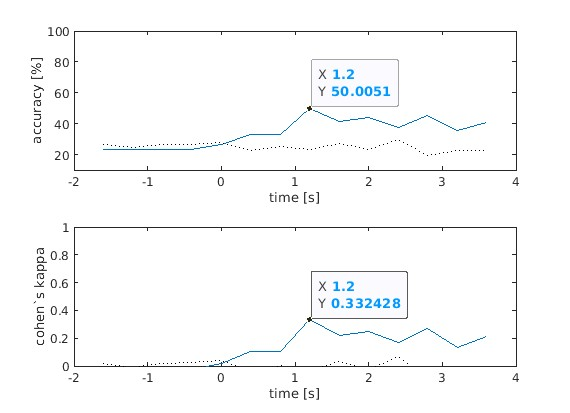
\includegraphics[width=\textwidth]{images/50.01-50hz-20-waveletCorrelation.jpg}
    \caption{This chart contains the performance measures of the Wavelet-Correlation-Feature extraction. This extraction method was tested with fs = 50Hz and a window size of 20 data-points.}
    %\label{fig:my_label}
\end{figure}

The correlation between EEG signals of each channel is statistically significant. Sub-sampling the data has high influence on the performance of the resulting model. Sub-sampling to low can lead to high information loss which decreases the overall performance of this extraction method. Selecting the right sub-sampling frequency is essential. 

\subsection{Wavelet-Entropy-Extractor}
Extraction of wavelet-entropy measure gets calculated on each data-point vector of the given window-size. The entropy extraction gets performed with different entropy measures and wavelet transform methods. The following parameters are permuted for determining the best configuration:

\begin{itemize}
    \item \textbf{Entropy Type:} Different entropy measures are used to calculate entropy (Shannon-, Renyi-, Tsallis-Entropy)
    \item \textbf{Transform Type:} The transform type that is used to calculate the wavelet coefficients (modwt, dwt, dwpt, modwpt)
    \item \textbf{fs:} Different sampling rates are used on the base eeg data. (250Hz, 50Hz, 25Hz)
    \item \textbf{Window Size:} Window sizes are adapted accordingly to the changed sampling rates (100, 20, 10)
\end{itemize}

Calculating the wavelet-entropy feature shows no high significance. As previously mentions in other methods, the entropy measure shows very bad performance. Optimizing different parameters only slightly improved performance. 

\subsection{Wavelet-Variance-Extractor}
This extractor calculates the variance of the wavelet coefficients of each time-domain data-point vector. The length of the data-point vector is equal to the window-size. The following parameters are permuted for determining the best configuration: 
\begin{itemize}
    \item \textbf{fs:} Different sampling rates are used on the base EEG data. (250Hz, 50Hz, 25Hz)
    \item \textbf{Window Size:} Window sizes are adapted accordingly to the changed sampling rates (100, 20, 10)
\end{itemize}

\begin{table}[H]
 \centering
 \begin{tabular}{|C{0.05\linewidth}|C{0.12\linewidth}|C{0.08\linewidth}|C{0.14\linewidth}|c|}
 \hline
   \textbf{fs [Hz]} & \centering\textbf{Window Size} & \textbf{Time [s]} & \textbf{Accuracy [\%]} & \textbf{Kappa} \\\hline
   50  & 20  & 1.2 & 51.20 & 0.348 \\
   250 & 100 & 1.2 & 46.85 & 0.290 \\
   25  & 10  & 1.2 & 38.90 & 0.185 \\\hline
 \end{tabular}
 \caption{Wavelet-Variance-Extractor performance comparison of different parameters}
 \label{tbl:wavelet-variance-feature-comparison-table}
 % Verweis im Text mittels \ref{tbl:wavelet-variance-feature-comparison-table}
\end{table} 

\begin{figure}[H]
    \centering
    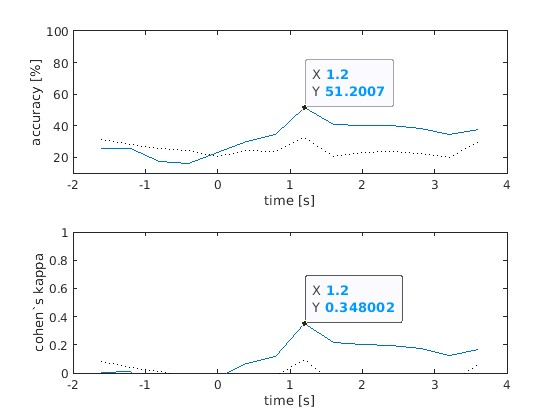
\includegraphics[width=\textwidth]{images/51.20-50hz-20-waveletVariance.jpg}
    \caption{This chart contains the performance measures of the Wavelet-Variance-Feature extraction. This extraction method was tested with fs = 50Hz and a window size of 20 data-points.}
    %\label{fig:my_label}
\end{figure}

The wavelet-variance feature is statistically highly significant and performs well on different sampling rates and the corresponding window sizes.

\section{Discussion}
Different feature extraction methods in the time- and frequency-domain were tested. Basically both work very well with the correct extraction method. Whereas frequency-domain feature extraction tend to have the high classification accuracies at a later time-point compared to time-domain feature extraction.

Extracting statistical features from time- or frequency-domain shows high classification performance. Especially when using the correct statistic measures. Statistic measures differ a little bit between the domains (Table \ref{tbl:domain-statistic-feature-comparison-table}). One large difference is the max-feature performs well only in the frequency spectrum.

\begin{table}[H]
 \centering
 \begin{tabular}{|C{0.5\linewidth}|C{0.4\linewidth}|}
 \hline
   \textbf{domain} & \textbf{statistic-features} \\\hline
   time (raw EEG data) & min, mean, median, std, prctile, slope \\
   frequency (Psd or Ar-Psd of raw EEG data) & min, max, mean, median, std, prctile, slope \\\hline
 \end{tabular}
 \caption{Comparison of good performing statistic features of different domains.}
 \label{tbl:domain-statistic-feature-comparison-table}
 % Verweis im Text mittels \ref{tbl:domain-statistic-feature-comparison-table}
\end{table} 

Ar-Coefficients show an high performance (around 45\%). Additionally it is important to select the correct order for the ar-model. If the order is to low or to high, the prediction would be based on to few or to many data-points and therefore will be incorrect. An order of 3 or 4 is sufficient and performs excellent.

Non promising features are the lyapunov exponents and the wavelet-entropy. The entropy measure performed overall very bad. It already showed in the statistic extractor that only small to no statistical significance is possible. Using the entropy for feature extraction might seem a good idea at first, but like the tests state perform very bad on the EEG of motor imagery.

The other two wavelet-extractors: wavelet-correlation and wavelet-variance performed tremendously good. Accuracies around 50\% show the high significance of this feature. Only the Ar-Psd extractor could achieve an higher classification performance (around 53\%).

EEG signal data can be compressed and extracted to different, smaller and still significant features. This improves training speed of models and enhances real-time EEG signal decoding. There is still room for improvement especially for parameter tuning. This report shows only a broad overview of the future potential of feature-engineering before feeding the data into a classifier.

\section{Conclusion}
Overall feature-engineering of EEG data is an important step to reduce the amount of data that is needed for training a model. This improves training performance and real-time EEG classification. Statistic extraction methods in the time and frequency domain, auto-regressive coefficients and wavelet extraction (correlation and variance) methods have been tested and show an incredible classification performance. There is still more effort to optimize the feature-extractors. Furthermore combining different feature of the feature-extractors should be tested in the future. 

\section{Further work/Recommendations}
Several feature extraction methods are described and compared. Eigenvector methods are not compared in this theses and should also be tested and compared. There is still room for improvement of parameter optimization of the feature-extractors. Combining multiple feature extractors should be performed in the future.

\section{Acknowledgements}
I would like to thank Kyriaki Kostoglou Pt. M.S. Ph.D. for giving helpful advice and feedback.

\printbibliography

\end{document}